\documentclass[11pt]{article}
\usepackage{amsmath,amssymb, amsthm, marvosym, permute, extsizes}
\usepackage{siunitx, graphicx, float, enumitem, adjustbox, hyperref, bm}
\usepackage{microtype, dsfont}
\usepackage[normalem]{ulem}
\usepackage[T1]{fontenc}
\usepackage[utf8]{inputenc}
\usepackage{lmodern}
\usepackage[T1]{fontenc}
\usepackage[a4paper,margin=2.5cm]{geometry}
\usepackage[icelandic]{babel}

\usepackage{minted}

\title{Heimadæmi 4\\ \vspace{0.4cm} \large Töluleg Greining}
\author{Emil Gauti Friðriksson}
\begin{document}
\maketitle
\section*{Dæmi 1}
Eftir að gefna forritinu hefur verið breytt þá fékkst eftirfarandi:
\begin{minted}{matlab}
function x_new=mymatitr(A,b,s)
[n,m]=size(A);
w=1.1;
assert(n == m && n == length(b));
x_old=zeros(n,1);
x_new=x_old;
for k=1:s
    for i=1:n
        x_new(i)=b(i);
        for j=1:n
            if j~=i
                %x_new(i)=x_new(i)-A(i,j)*x_old(j); % Jacobi
                 x_new(i)=x_new(i)-A(i,j)*x_new(j); % Gauss-Seidel
            end
        end
        x_new(i)=x_new(i)/A(i,i);
        x_new(i)=(1-w)*x_old(i) + w*x_new(i);%sleppa þessari fyrir Gauss-Seidel        
    end
    x_old=x_new;
end
end
\end{minted}
Niðurstöður forrits með gefnum gildum í dæminu skilaði sömu niðurstöðum og bókin hefur.

\newpage
\section*{Dæmi 2}
\subsection*{Dæmi 8(b) úr 2.6 Exercises}
Solve the system of equations by finding the Cholesky factorization of A followed by two back
substitutions.
$$
\begin{bmatrix}
4 & -2 & 0\\
-2 & 2 & -1\\
0 & -1 & 5
\end{bmatrix}
\begin{bmatrix}
x_1\\
x_2\\
x_3
\end{bmatrix}
=
\begin{bmatrix}
0\\
3\\
-7
\end{bmatrix}
$$
\subsection*{Svar}
Fyrsta stakið í R er $R_{11} = \sqrt[]{4} = 2$ og síðan eru $R_{1,2} = \frac{-2}{R_{11}} = -1$ og $R_{1,3} = \frac{0}{R_{11}} = 0$
og fáum þá að 
$uu^T = 
\begin{bmatrix}
-1\\
0
\end{bmatrix}
\begin{bmatrix}
-1 & 0
\end{bmatrix}
=
\begin{bmatrix}
1 & 0\\
0 & 0
\end{bmatrix}
$
 Sem við drögum frá $A_{2:3,2:3}$ og fáum 
 $R_{2,2} = \sqrt[]{A_{2,2} - 1} = 1$ og $R_{2,3} = (A_{2,3} - 0)/1 = -1$.
 Nú er $R_{33} = \sqrt[]{5-(-1)(-1)} = 2$\\
Því fáum við 
$$
R=
\begin{bmatrix}
2 & -1 & 0\\
0 & 1 & -1\\
0 & 0 & 2
\end{bmatrix}
$$
Athugum nú hvort þetta sé rétt
$$
R^TR = 
\begin{bmatrix}
2 & 0 & 0\\
-1& 1 & 0\\
0 & -1& 2
\end{bmatrix}
\begin{bmatrix}
2 & -1 & 0\\
0 & 1 & -1\\
0 & 0 & 2
\end{bmatrix}
=
\begin{bmatrix}
4 & -2 & 0\\
-2 & 2 & -1\\
0 & -1 & 5
\end{bmatrix}
$$
Mergjað!\\
Við skulum nú finna gildin á [$x_1, x_2, x_3$]. Athugum því $R^Tc = b$
$$
\begin{bmatrix}
2 & 0 & 0\\
-1& 1 & 0\\
0 &-1 & 2
\end{bmatrix}
\begin{bmatrix}
c_1\\
c_2\\
c_3
\end{bmatrix}
=
\begin{bmatrix}
0\\
3\\
-7
\end{bmatrix}
$$
Fáum úr þessu gildin $[c_1, c_2, c_3] = [0, 3, -2]$ Athugum þá $Rx=c$
$$
\begin{bmatrix}
2 & -1 & 0\\
0 & 1  & -1\\
0 & 0 & 2
\end{bmatrix}
\begin{bmatrix}
x_1\\
x_2\\
x_3
\end{bmatrix}
=
\begin{bmatrix}
0\\
3\\
-2
\end{bmatrix}
$$
úr þessu fæ ég gildin: $[x_1,x_2,x_3] = [1,2,-1]$

\subsection*{Dæmi 13(a) úr 2.6 Exercises}
Solve the problems by carrying out the Conjugate Gradient Method by hand.
$$
\begin{bmatrix}
1 & 2\\
2 & 5
\end{bmatrix}
\begin{bmatrix}
u\\
v
\end{bmatrix}
=
\begin{bmatrix}
1\\
1
\end{bmatrix}
$$
\subsection*{Svar}
Athugum að rétt svar(fundið með hefðbundum fylkjaruðning) er $[u,v]=[3,-1]$
Áður en við hefjum reikninga, ákveðum að velja upphafsgildin okkar $x_0 = [0,0]$ og þá $r_0 = b = [1,1]$.\\
Hefjum leikana:
\begin{align*}%lína 1
\alpha_0 = \frac{r_0^Tr_0}{d_0^TAd_0} = \frac{\begin{bmatrix}
1 & 1
\end{bmatrix}
\begin{bmatrix}
1\\1
\end{bmatrix}}{\begin{bmatrix}
1 & 1
\end{bmatrix}\begin{bmatrix}
1 & 2\\
2 & 5
\end{bmatrix}
\begin{bmatrix}
1\\1
\end{bmatrix} }
=\frac{1}{5}
\end{align*}

\begin{align*} %Lína 2
x_1 = x_0 + d_0 + \alpha d_0 = 1/5\begin{bmatrix}1\\1\end{bmatrix}
\end{align*}

\begin{align*} %lína 3
r_1 = r_0-\alpha_0Ad_0 = \begin{bmatrix}1\\1\end{bmatrix}-1/5
\begin{bmatrix}
1 & 2\\
2 & 5
\end{bmatrix}
\begin{bmatrix}
1\\1
\end{bmatrix}
=
1/5
\begin{bmatrix}
-2\\2 
\end{bmatrix}
\end{align*}

\begin{align*}% lína 4
\beta_0 = \frac{r_1^T r_1}{r_0^Tr_0} = \frac{2\cdot (2/5)^2}{2} = \frac{4}{25}
\end{align*}

\begin{align*}% lína 5
d_1 = r_1 + \beta_0d_0 = 1/5 \begin{bmatrix}
2\\-2
\end{bmatrix}
(4/25)\begin{bmatrix}
1\\1
\end{bmatrix}
= (2/25)\begin{bmatrix}
7\\-3
\end{bmatrix}
\end{align*}

\begin{align*} %lína 6
\alpha_1 = \frac{r_1^Tr_1}{d^TAd_1} = \frac{(1/25)*2^3}{(2/25)^2 \begin{bmatrix}
7 & -3
\end{bmatrix} \begin{bmatrix}
1 & 2 \\
2 & 5
\end{bmatrix}
\begin{bmatrix}
7\\-3
\end{bmatrix}}
= \frac{8}{\frac{4}{25}\cdot 10} = 5
\end{align*}

\begin{align*} % lína 7
x_2 = x_1 + \alpha_1d_1 = (1/5)\begin{bmatrix}
1\\1
\end{bmatrix}
+5 \frac{2}{25}
\begin{bmatrix}
7\\-3
\end{bmatrix}
=
\frac 15
\begin{bmatrix}
15\\-5
\end{bmatrix}
=
\begin{bmatrix}
3\\-1
\end{bmatrix}
\end{align*}
Þetta er sama svar og við fengum í upphafi dæmisins.

\newpage
\section*{Dæmi 3}
\subsection*{Dæmi 3(a) úr 2.7 Exercises}
Sketch the two curves in the uv-plane, and find all solutions exactly by simple algebra.
$$
\begin{cases}
u^2+v^2=1\\
(u-1)^2+v^2=1
\end{cases}
$$
\subsection*{Svar}
Teiknum mynd af þessum tveim ferlum:
\begin{figure}[h]
\centering
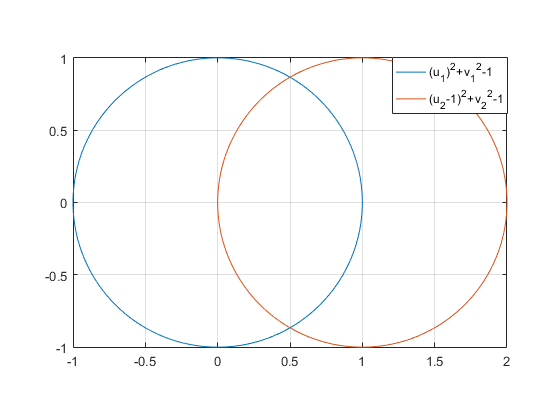
\includegraphics[scale=0.8]{mynd433.png}
\end{figure}\\
Byrjum á að draga línu 1 frá línu 2 og fáum þá
\begin{align*}
(u-1)^2-u^2 	&= 0\\
	-2u+1		&= 0\\
\Rightarrow u 	&= \frac 12\quad\text{Stingum  inn í efri jöfnuna}\\
\frac 14 + v^2 	&= 1\\
\Rightarrow v 	&= \pm \sqrt[]{\frac 34}
\end{align*}
Sjáum að niðurstöðurnar okkar fyrir skurðpunkta hringjanna tveggja er $[u_1,v_1] = [\frac 12, \sqrt[]{\frac 34}]$ og $[u_2,v_2]=[\frac 12, -\sqrt[]{\frac 34}]$ sem er í samræmi við mynd.


\subsection*{Dæmi 4 úr 2.7 Exercises}
Apply two steps of Newton’s Method to the systems in Exercise 3, with starting point (1,1).
\subsection*{Svar}
Höfum $DF(x) = \begin{bmatrix}
2u & 2v\\
2(u-1) & 2v
\end{bmatrix}$.\\
Við viljum leysa þegar búið er að stinga $x_0$ inn í $DF(x)$:
\begin{align*}
\begin{bmatrix}
2 & 2\\
0 & 2
\end{bmatrix}
\begin{bmatrix}
s_1\\
s_2
\end{bmatrix}
=
\begin{bmatrix}
-1\\
0
\end{bmatrix}
\end{align*}
Sem hefur lausnina $s=\begin{bmatrix}
s_1\\s_2
\end{bmatrix} = \begin{bmatrix}
-1\\0
\end{bmatrix}$
því fáum við að $x_1 = x_0 +s =\begin{bmatrix}
\frac 12\\1
\end{bmatrix}$\\
Byrjum ferlið aftur en nú notum við $x_1$\\
Viljum því leysa:
\begin{align*}
\begin{bmatrix}
1 & 2\\
-1& 2
\end{bmatrix}
\begin{bmatrix}
s_1\\s_2
\end{bmatrix}
=
\begin{bmatrix}
-\frac 14\\
-\frac 14
\end{bmatrix}
\end{align*}
sem hefur lausnina $s=\begin{bmatrix}
s_1\\s_2
\end{bmatrix}= \begin{bmatrix}
0\\-\frac 18
\end{bmatrix}$\\
Því fáum við $x_2 = x_1 + s = \begin{bmatrix}
\frac 12\\1
\end{bmatrix}
+ \begin{bmatrix}
0\\-\frac 18
\end{bmatrix}
= \begin{bmatrix}
\frac 12\\ \frac 78
\end{bmatrix}$
Sjáum að þetta er ekki alveg rétt, $\frac 78 \neq \sqrt[]{\frac 34}$ en er þó ágætis nálgun.




\subsubsection*{Dæmi 5 úr 2.7 Exercises}
Apply two steps of Broyden I to the systems in Exercise 3, with starting point (1,1), using
A0 = I .
\subsection*{Svar}














\end{document}
